% !TEX program = lualatex
%==============================================================================
% プリアンブル (Preamble)
%==============================================================================

\documentclass[a4paper, 11pt]{ltjsarticle}

%------------------------------------------------------------------------------
% パッケージ読み込み
%------------------------------------------------------------------------------
\usepackage[margin=2.5cm]{geometry}
\usepackage{amsmath}           % 数式
\usepackage{booktabs}          % 表
\usepackage{siunitx}           % 単位
\usepackage{graphicx}          % 画像読み込み
\usepackage{float}             % 画像配置の制御
\usepackage{luatexja-fontspec} % 和文フォント
\usepackage{listings}          % ソースコード
\usepackage{xcolor}            % 色

% listings の設定
\lstset{
	basicstyle=\ttfamily\small,
	keywordstyle=\color{blue}\bfseries,
	commentstyle=\color{green!40!black},
	stringstyle=\color{red!60!black},
	numbers=left,
	numberstyle=\tiny,
	stepnumber=1,
	numbersep=5pt,
	frame=single,
	breaklines=true,
	breakatwhitespace=true,
	columns=fullflexible,
	showstringspaces=false,
	language=Python,
	inputencoding=utf8,
	captionpos=b
}

%------------------------------------------------------------------------------
% 各種設定
%------------------------------------------------------------------------------

% --- 和文フォント設定 ---
\setmainjfont[Renderer=HarfBuzz]{Yu Mincho}
\setsansjfont[Renderer=HarfBuzz]{Yu Gothic}

% --- ドキュメント情報 ---
\title{画像処理・画像処理工学 レポート課題1}
\author{画像処理工学科 学籍番号: 21239 組番号:234 5E 氏名:栁原 魁人}
\date{\today}

%==============================================================================
% ドキュメント本体 (Body)
%==============================================================================
\begin{document}

\maketitle
\thispagestyle{empty}
\clearpage

\section{課題1}

\subsection{問題1-1: メディアンカット量子化法}

\subsubsection{理論}
ピクセル値をソートして目標色数のグループに均等分割し、各グループの中央値を代表色として設定する手法。

\subsubsection{計算・導出過程}

図A-1に示す4×5画素の画像に対してメディアンカット量子化法を適用し、4色に量子化します。

全ピクセル値:
\begin{center}
	102, 179, 92, 14, 106, 74, 202, 87, 116, 99, 151, 130, 149, 52, 1, 235, 157, 37, 129, 191
\end{center}

ソート:
\begin{center}
	1, 14, 37, 52, 74, 87, 92, 99, 102, 106, 116, 129, 130, 149, 151, 157, 179, 191, 202, 235
\end{center}

4つのグループに均等分割(各5ピクセル):

\begin{table}[H]
	\centering
	\begin{tabular}{|c|c|c|}
		\hline
		グループ & ピクセル値 & 代表色(中央値) \\
		\hline
		1 & 1, 14, \textbf{37}, 52, 74 & 37 \\
		2 & 87, 92, \textbf{99}, 102, 106 & 99 \\
		3 & 116, 129, \textbf{130}, 149, 151 & 130 \\
		4 & 157, 179, \textbf{191}, 202, 235 & 191 \\
		\hline
	\end{tabular}
\end{table}

量子化結果:
\begin{center}
	\begin{tabular}{|c|c|c|c|c|}
		\hline
		99 & 191 & 99 & 37 & 99 \\
		\hline
		37 & 191 & 99 & 130 & 99 \\
		\hline
		130 & 130 & 130 & 37 & 37 \\
		\hline
		191 & 191 & 37 & 130 & 191 \\
		\hline
	\end{tabular}
\end{center}

\subsubsection{結果}

\begin{figure}[H]
	\centering
	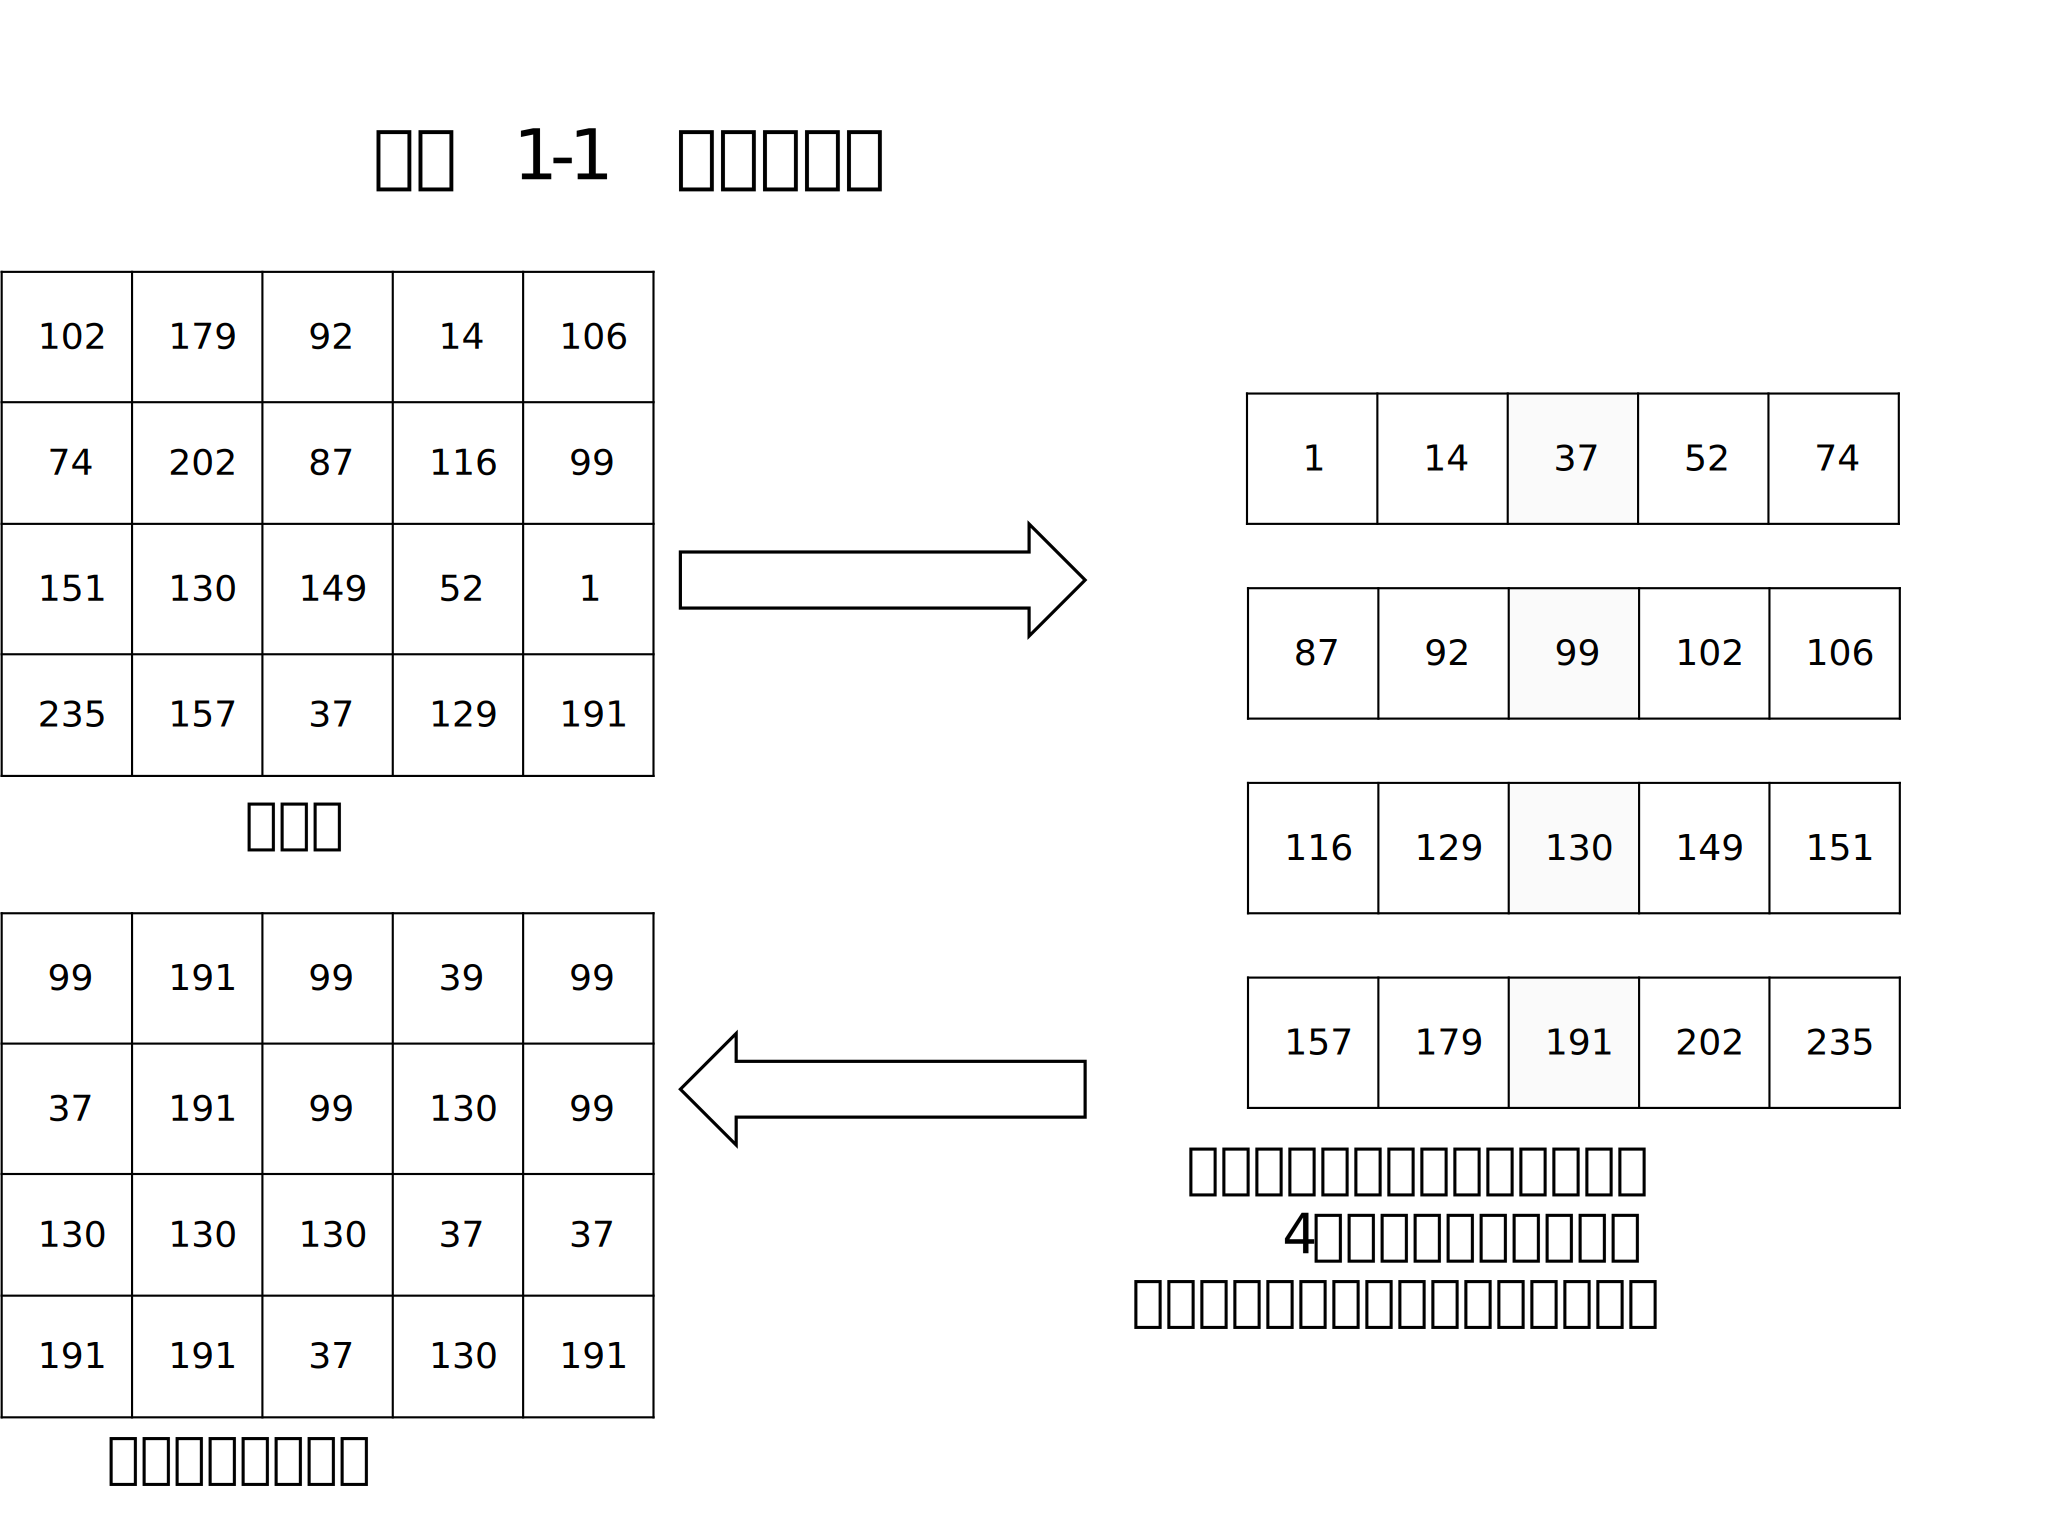
\includegraphics[width=0.85\textwidth]{問題1-1.pdf}
	\caption{メディアンカット量子化の結果}
	\label{fig:median_cut}
\end{figure}

\clearpage

\subsection{問題1-2: ラベリング処理}

\subsubsection{理論}
2値画像で連結成分に同一ラベルを割り当てる。2回走査法:第1回で仮ラベル割当と等価関係記録、第2回で統合。

\subsubsection{計算・導出過程}

図A-2の10×10画素画像に対してラベリングを実行。

第1回走査:左上から右下へ走査。各白ピクセルについて左上・上・右上・左を確認。
\begin{itemize}
	\item 全て黒 → 新規ラベル割当
	\item いずれかが白 → そのラベル継承
	\item 複数が異なるラベル → 最小値割当、等価関係記録
\end{itemize}

等価ラベル関係:$A - B - C$, $E - F$, $D$

第2回走査:等価関係に基づいて代表ラベルに統一。

\begin{table}[H]
	\centering
	\begin{tabular}{|c|c|c|}
		\hline
		仮ラベル & 等価関係 & 代表ラベル \\
		\hline
		A, B, C & $A - B - C$ & A \\
		D & 単独 & D \\
		E, F & $E - F$ & E \\
		\hline
	\end{tabular}
\end{table}

\subsubsection{結果}

\begin{figure}[H]
	\centering
	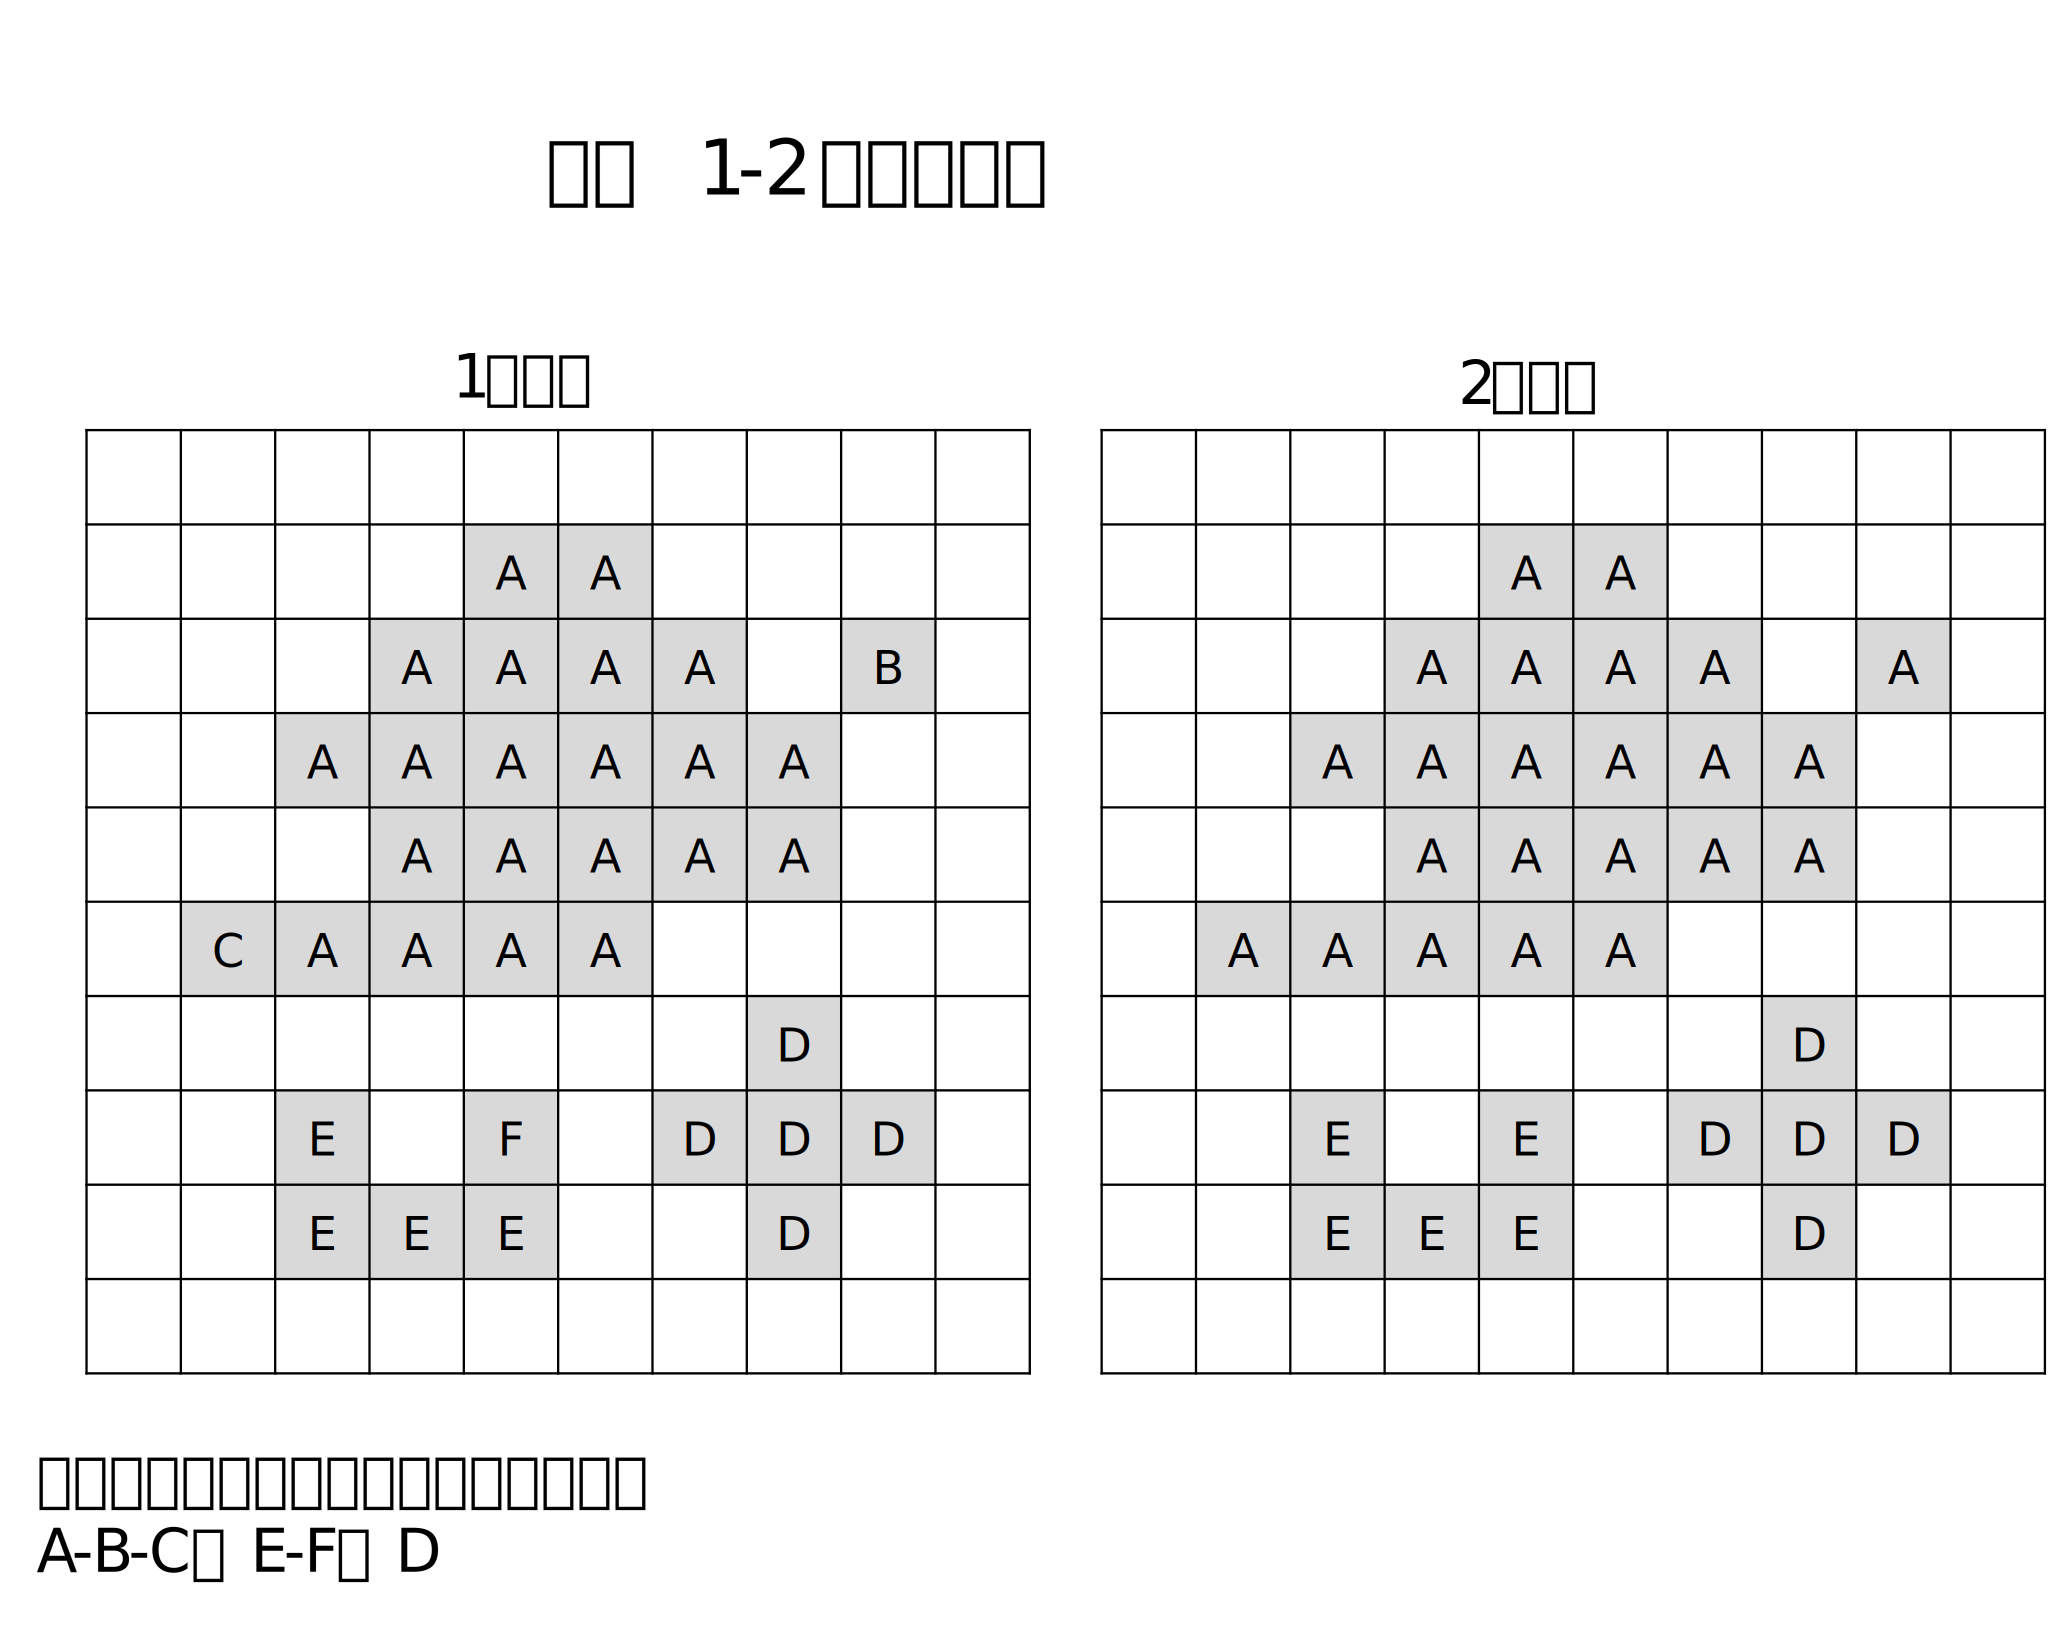
\includegraphics[width=0.9\textwidth]{問題1-2.pdf}
	\caption{ラベリング処理の結果}
	\label{fig:labeling}
\end{figure}

\clearpage

\subsection{問題1-3: ハフマン符号化}

\subsubsection{理論}
高確率シンボルに短い符号を割り当てる可変長符号化。ハフマン木を構築して符号を生成。

\subsubsection{計算・導出過程}

8シンボルの出現確率:

\begin{table}[H]
	\centering
	\begin{tabular}{|c|c|c|}
		\hline
		シンボル & 確率 & 符号 \\
		\hline
		0 & 0.30 & 10 \\
		1 & 0.02 & 00001 \\
		2 & 0.06 & 0011 \\
		3 & 0.04 & 0001 \\
		4 & 0.01 & 00000 \\
		5 & 0.05 & 0010 \\
		6 & 0.20 & 01 \\
		7 & 0.32 & 11 \\
		\hline
	\end{tabular}
\end{table}

		結合ステップ(低い確率から順に):
		\begin{enumerate}
			\item 4(0.01)+1(0.02)=0.03 → A
			\item A(0.03)+3(0.04)=0.07 → B
			\item 5(0.05)+2(0.06)=0.11 → C
			\item B(0.07)+C(0.11)=0.18 → D
			\item D(0.18)+6(0.20)=0.38 → E
			\item 0(0.30)+7(0.32)=0.62 → F
			\item E(0.38)+F(0.62)=1.00 → Root
		\end{enumerate}

平均符号長計算:
\begin{align*}
L &= 0.30 \times 2 + 0.02 \times 5 + 0.06 \times 4 + 0.04 \times 4 \\
  &\quad + 0.01 \times 5 + 0.05 \times 4 + 0.20 \times 2 + 0.32 \times 2 \\
  &= 2.39 \text{ bits/シンボル}
\end{align*}

等長符号(3 bits/シンボル)との比較:削減量 $= 3 - 2.39 = 0.61$ bits(約20\%削減)

\subsubsection{結果}

\begin{figure}[H]
	\centering
	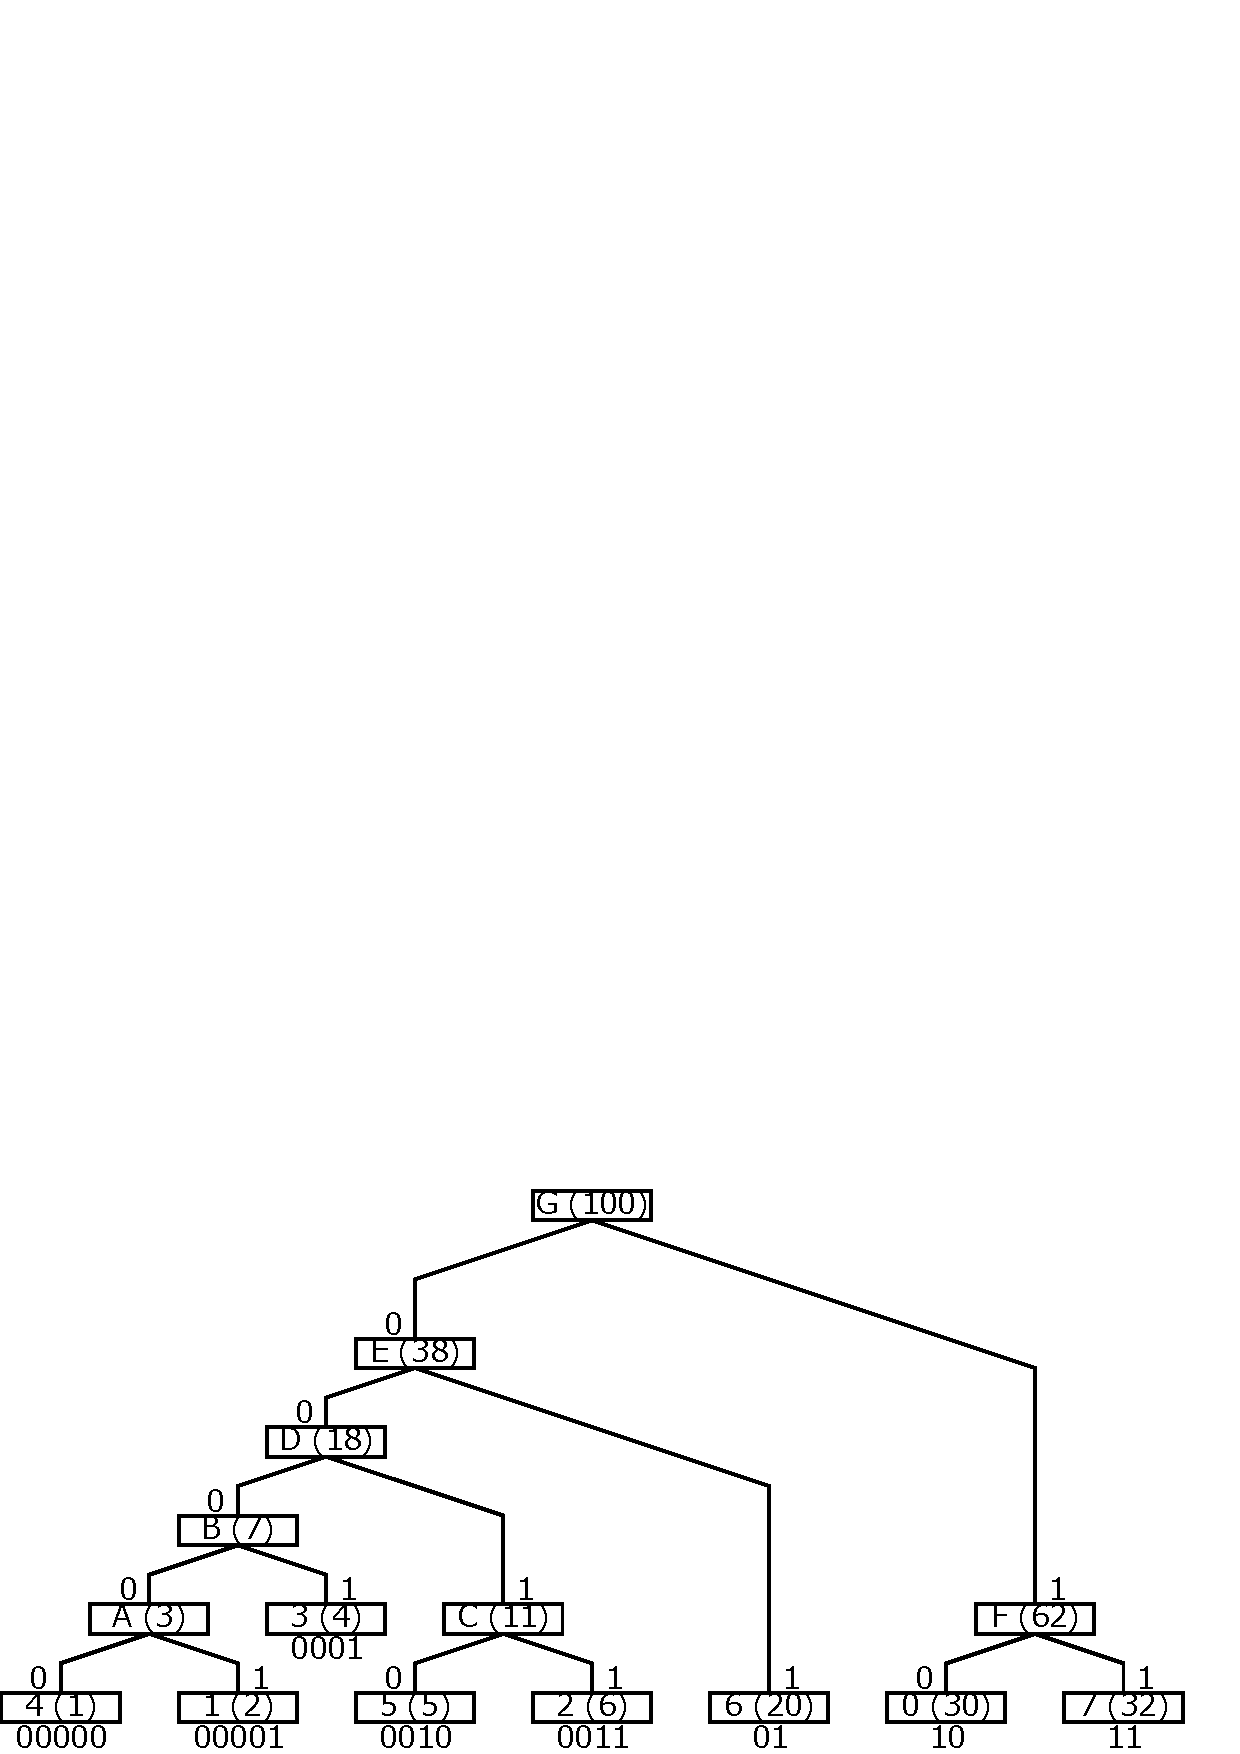
\includegraphics[width=0.8\textwidth]{問題1-3.pdf}
	\caption{ハフマン木の構造}
	\label{fig:huffman}
\end{figure}

\clearpage

\section{課題2}

\section{問題1: モルフォロジー処理によるノイズ除去}

\subsection{概要}
開処理と閉処理を用いてノイズを除去。

\subsection{結果}
開処理により小さなノイズ除去、閉処理により黒いノイズを埋め込み。

\begin{figure}[H]
	\centering
	\includegraphics[width=0.95\textwidth]{a2-3_binary_image_kernel_size_15.png}
	\caption{Kernel size 15 での開閉処理結果(ノイズ除去後の2値画像)}
	\label{fig:morph_kernel15}
\end{figure}

	カーネルサイズ9以降は見た目の変化が小さく、9で十分。15にする必然性はない。

\clearpage

\section{問題2: JPEG品質と圧縮率の関係}

\subsection{概要}
JPEG品質と圧縮率、SSIM値の関係を調査。

\subsection{結果}
下表は本レポートで得られた数値(品質Q、サイズ比、SSIM)を整理したもの。

\begin{table}[H]
\centering
\caption{品質Qによるサイズ比とSSIM}
\label{tab:jpeg_q_ssim}
\begin{tabular}{rcc}
\toprule
Q & サイズ比(\%) & SSIM \\
\midrule
0   & 0.9  & 0.327 \\
10  & 2.2  & 0.520 \\
20  & 3.6  & 0.609 \\
30  & 4.8  & 0.656 \\
40  & 5.8  & 0.686 \\
50  & 6.7  & 0.709 \\
60  & 7.7  & 0.729 \\
70  & 9.3  & 0.753 \\
80  & 11.8 & 0.783 \\
90  & 17.7 & 0.825 \\
100 & 45.5 & 0.871 \\
\bottomrule
\end{tabular}
\end{table}

\begin{figure}[H]
\centering
\includegraphics[width=0.95\textwidth]{a2-4_color_image_jpeg_compression_analysis.png}
\caption{JPEG品質Qごとの視覚比較とサイズ比・SSIM(提示画像)}
\label{fig:jpeg_q_grid}
\end{figure}

\textbf{Q=80} でSSIM=0.783、\textbf{Q=90} でSSIM=0.825 と向上するが、サイズ比は 11.8\%→17.7\%へ増加。視覚・数値の両面から、実用的には \textbf{Q=80~90} が妥当。\textbf{Q=100} はSSIM向上が小さい一方でサイズ比 45.5\% と非効率。

\clearpage

\section{問題3: 2次元FFTと振幅スペクトル}

\subsection{概要}
グレースケール画像を2次元FFTで周波数領域に変換し、振幅スペクトルを分析。

\subsection{結果}

\begin{figure}[H]
\centering
\includegraphics[width=0.85\textwidth]{a2-5_gray_image_magnitude_spectrum_combined_fft_plots.png}
\caption{グレースケール画像の2次元振幅スペクトル(中央化)}
\label{fig:fft_magnitude}
\end{figure}

振幅スペクトルの中心に強い明るさを示す領域がある。これはDC成分(0周波数)と低周波成分が画像の主要成分であることを示す。周辺部は暗く、高周波成分(細かなエッジやノイズ)が少ないことを表す。垂直・水平方向に弱い構造が見られるのは、画像内に規則的な境界や勾配が存在することを示唆している。

\clearpage

\section{問題4: 周波数フィルタの応用}

\subsection{概要}
理想的ローパスフィルタ(ILPF)とガウシアンハイパスフィルタ(GHPF)をCutoff=30で適用し、効果を比較。

\subsection{結果}

\begin{figure}[H]
\centering
\includegraphics[width=0.95\textwidth]{a2-5_gray_image_output_filters_result.png}
\caption{ローパスフィルタとハイパスフィルタの適用結果比較(Cutoff=30)}
\label{fig:filter_comparison}
\end{figure}

\textbf{ローパスフィルタ(ILPF)}: 低周波成分のみを通し、高周波(ノイズ・細部)を除去。結果は全体的にぼかされ、目や顔の大型構造は保持される一方、毛並みなどの細かいテクスチャは消失。ノイズ除去やスムージングに有効。

\textbf{ハイパスフィルタ(GHPF)}: DC成分と低周波を除去し、高周波のみを通す。結果はエッジが明るく浮き出ち、目・口・毛並みなどの細部が強調される。大きな領域は暗くなり、画像全体はコントラストが低下。エッジ検出と細部抽出に有効。

\clearpage

\section*{付録: プログラムリスト}

\subsection*{問題1: モルフォロジー処理}

\lstinputlisting[caption={問題1 モルフォロジー処理によるノイズ除去}, label={lst:code1}, language=Python]{../問題2_1.py}

\clearpage

\subsection*{問題2: JPEG品質と圧縮率}

\lstinputlisting[caption={問題2 JPEG品質と圧縮率の関係調査}, label={lst:code2}, language=Python]{../問題2_2.py}

\clearpage

\subsection*{問題3: 2次元FFTと振幅スペクトル}

\lstinputlisting[caption={問題3 2次元FFTと振幅スペクトル}, label={lst:code3}, language=Python]{../問題2_3.py}

\clearpage

\subsection*{問題4: 周波数フィルタの応用}

\lstinputlisting[caption={問題4 周波数フィルタの応用}, label={lst:code4}, language=Python]{../問題2_4.py}

\end{document}
